% ----------------------------------------------------------
\chapter{Systematic Review of the Literature: Text Representation}\label{ap:rsl_representation_law}
% ----------------------------------------------------------


% - Focus on word embeddings and language models
% - 

In this SRL, we tried to find work related to the application of text representation techniques on legal texts written in the Portuguese language. However, such task did not succeed due to the absence of work in that sense. Thus, two smaller SRLs were conducted to find papers with broader searches. The first focused on the representation of legal texts in any language and the second in the representation of general texts in Portuguese. 

\section{Definition of Search Questions}

The question of the first search: ``What are the text representation techniques applied to texts from the legal domain?''

The question of the second search: ``What are the text representation techniques applied to texts written in Portuguese?''

\section{Search Strategies}

Search for representation of legal texts in any languages:

\begin{verbatim}
("legal" OR "law" OR "court" OR "justice") AND ("embedding*" OR 
"language model*" OR "machine learning" OR "deep learning" OR 
"natural language processing" OR "text mining") AND ("doc2vec" 
OR "paragraph2vec" OR "word2vec" OR "glove" OR "wang2vec" OR 
"fasttext" OR "bert" OR "elmo" OR "law2vec")
\end{verbatim}


Search for representation of general texts in Portuguese:

\begin{verbatim}
("portuguese" OR "brazil*") AND ("embedding*" OR "deep learning" OR 
"machine learning" OR "natural language processing" OR "text mining") 
AND ("doc2vec" OR "paragraph2vec" OR "word2vec" OR "glove" OR 
"wang2vec" OR "fasttext" OR "bert" OR "elmo" OR "law2vec" ) 
\end{verbatim}



\section{Knowledge Bases}

In this SRL, we searched on the following bases:

\begin{itemize}[noitemsep]
    \item Scopus
    \item ACM Digital Library
    \item IEEE Xplore
    \item Web of Science
\end{itemize}


\section{Inclusion and Exclusion Criteria}


Following the questions of this research, we defined a set of inclusion and exclusion criteria. The process of selection embraced the reading of title, abstract and keywords and the accordance with the criteria:

The following is the list of inclusion criteria:

\begin{itemize}[noitemsep]
    \item Published in journal or conference
    \item Involves legal texts in any languages or general texts in Portuguese;
    \item Involves Machine Learning or Text Mining;
    \item The techniques used are named;
    \item The work evaluate or train representations
    \item Empirical Work;
    \item Published from 2010 and May 2020.
\end{itemize}

And the following is the list of exclusion criteria:

\begin{itemize}[noitemsep]
    \item Work not written in Portuguese or English;
    \item Published over 10 years ago;
    \item Does not involve legal texts in any language neither general texts in Portuguese;
    \item Does not involve Machine Learning or Text Mining;
    \item Theoretic work
\end{itemize}

\section{Data Extraction Plan}

In the SRL from this section, we focused on just retrieving the representation techniques used and the application.

\section{Search Execution and Preliminary Analysis}

After applying the first search string to the knowledge base on May 7, 2020 for researches published from 2010 to May 2020, the search returned 52 documents. After reading title, abstract and keywords and applying the selection criteria, the number of papers reduced to 12.

In terms of the second search string, after applying to the knowledge base on May 7, 2020 with the same time filtering, the search returned 136 documents. After reading title, abstract and keywords and applying the selection criteria, the number of papers reduced to 20.


\section{Results and Analysis}

In this section, we show the results and analysis in terms of representation techniques for the first part of this SRL related to legal texts from many languages and general texts in Portuguese.

In the first part of this research, we focused on the representation techniques applied in the legal domain. In Figure \ref{fig:rsl_legal_representation}, one can see the distribution by year of the research interest, on the area of representation of legal documents for ML tasks, considering our selection criteria. Although we set the interval to ten years, the selected work only embraced three distinct years.


\begin{figure}[htb]
    \centering
    \caption{Researches by year for text representation in legal documents}
    \label{fig:rsl_legal_representation}
    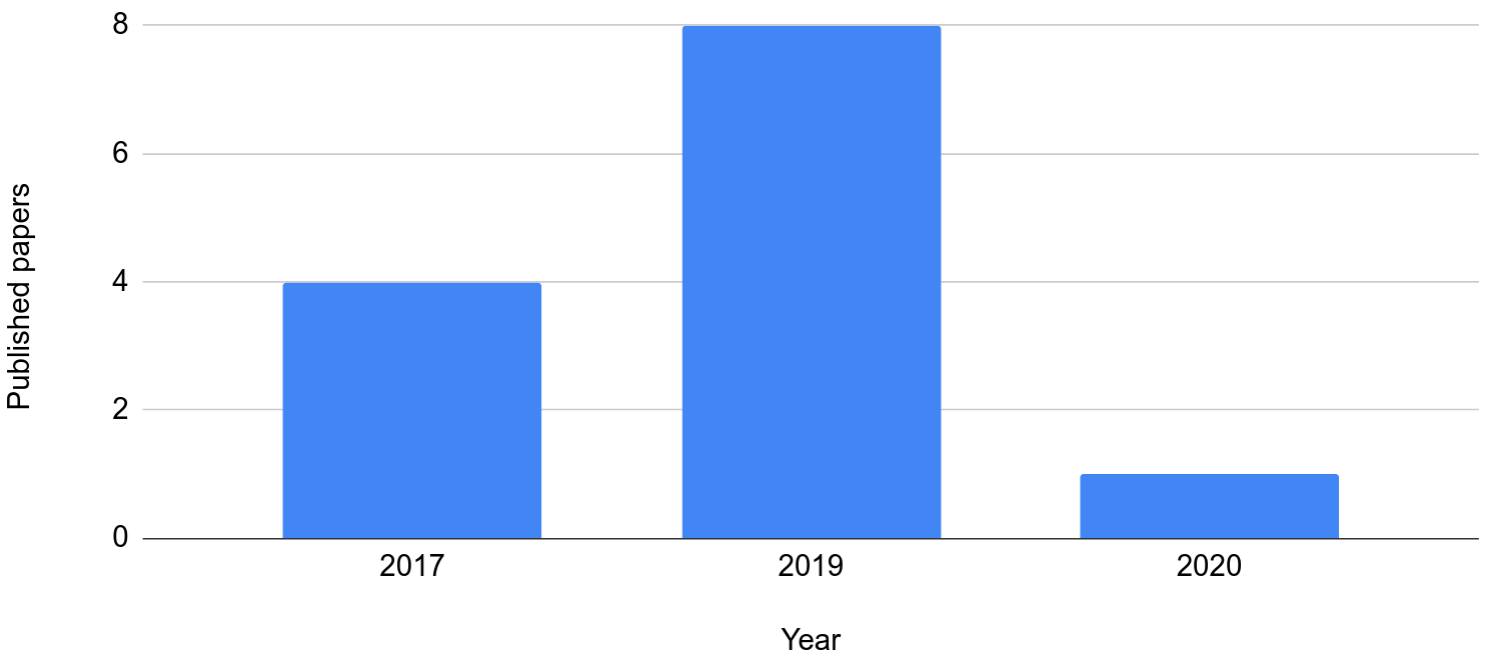
\includegraphics[width=\textwidth]{images/appendix/rsl_legal_representation.png}
\end{figure}

In Table \ref{tab:rsl_representation_legal}, there is the list of representation techniques used in the selected work. Note that, many papers reported using more than one representation techniques in their experiments.

% Most frequent Representations
\begin{table}[htb]
\centering
\caption{Representations applied to legal texts}
\label{tab:rsl_representation_legal}
\footnotesize
\begin{tabular}{cc}
\hline
\textbf{Representation} & \textbf{Papers} \\ \hline
Word2Vec                & 8               \\
Doc2Vec                 & 2               \\
WordVec CBOW           & 2               \\
Glove                   & 2               \\
FastText                & 2               \\
ELMo                    & 1               \\
Bag of Words            & 1               \\
Law2Vec                 & 1              \\\bottomrule
\end{tabular}
\end{table}

In the second part of this research, we focused on the representation techniques applied in general texts written in the Portuguese language. In Figure \ref{fig:rsl_representation_portuguese_year}, one can see the distribution by year of the research interest on the area, considering our selection criteria. Although, the SRL embraced the last ten years the selected work embraced the last five.


\begin{figure}[htb]
    \centering
    \caption{Researches by year for text representation in Portuguese documents}
    \label{fig:rsl_representation_portuguese_year}
    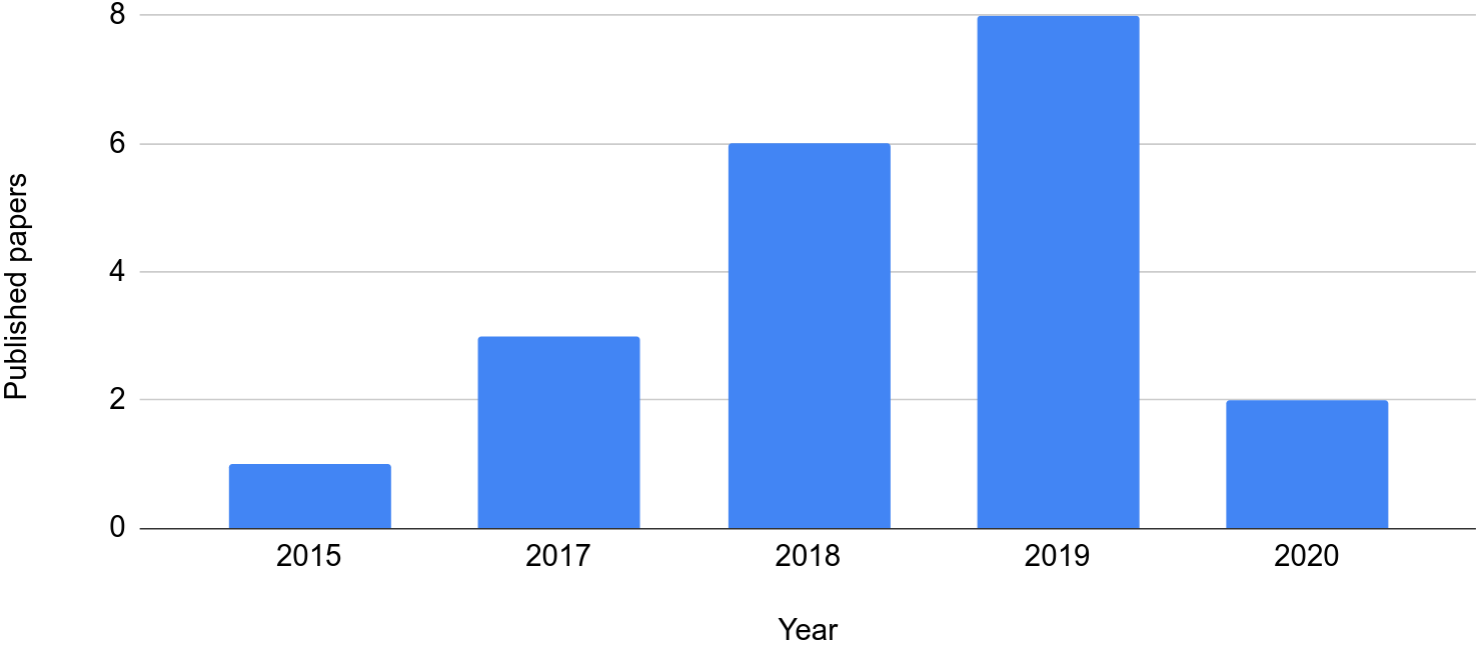
\includegraphics[width=\textwidth]{images/appendix/rsl_portuguese_representation.png}
\end{figure}

In Table \ref{tab:rsl_representation_portuguese}, there is the list of representation techniques used in the selected work. Note that, many papers reported using more than one representation techniques in their experiments.

\begin{table}[htb]
\centering
\caption{Representation used in Portuguese texts}
\label{tab:rsl_representation_portuguese}
\footnotesize
\begin{tabular}{cc}
\hline
\textbf{Representation} & \textbf{Papers} \\ \hline
Word2Vec                & 7               \\
Word2Vec Skipgram       & 7               \\
Glove                   & 6               \\
TF-IDF                  & 3               \\
Wang2Vec Skipgram       & 3               \\
Bag of Words            & 2               \\
ELMo                    & 2               \\
FastText                & 2               \\
FastText Skipgram       & 2               \\
LDA                     & 2              \\ \bottomrule
\end{tabular}
\end{table}

% Tasks

As mentioned, we do not find, until the date of the SRLs, any work related to evaluation or training of representations of  legal texts in the Portuguese language.

